% Intended LaTeX compiler: pdflatex
\documentclass[10pt,a4paper,UTF8]{article}
\usepackage{zclorg}
\usepackage{tikztheorem}
\author{zcl.space}
\date{}
\title{二项随机变量}
\hypersetup{
 pdfauthor={zcl.space},
 pdftitle={二项随机变量},
 pdfkeywords={probability},
 pdfsubject={},
 pdfcreator={Emacs 25.0.50.1 (Org mode 9.0.6)},
 pdflang={English}}
\begin{document}

\maketitle
\tableofcontents
\titlepic{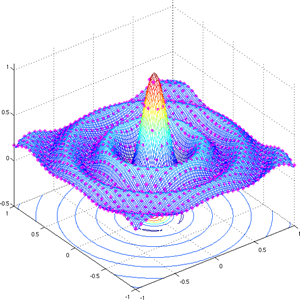
\includegraphics[scale=0.25]{../../img/sinc.PNG}}


\section{伯努利随机变量和二项随机变量}
\label{sec:org98f4d9f}


假定一个实验,其结果可以分为成功或者失败。如果我们在试验的机故宫是成功时令\(X=1\),而在试验的结果是失败时令\(X=0\),那么\(X\)的概率质量函数是:
\begin{eqnarray}
\label{eq:1}
p(0)&=&P(X = 0) = 1-p \\
p(1)&=&P(X = 1) = p
\end{eqnarray}

其中\(p,0\leq p \leq 1\)是试验的结果为成功的概率。

随机变量\(X\)成为伯努利随机变量,如果其概率密度函数由式(\ref{eq:1})给出. 现在我们推广伯努利随机变量。

假定做了\(n\) 次试验,其中每次结果成功的概率为\(p\),失败的概率为\(1-p\),如果以\(X\)代表出现在\(n\)次试验中成功的次数,那么\(X\)称为具有参数\((n,p)\)的二项随机变量,其概率质量函数为:
\begin{equation}
\label{eq:2}
p(i) = \binom{n}{i}p^{i}(1-p)^{n-i}, i = 0,\ldots ,n
\end{equation}
可以通过二项式定理验证,这些概率加起来是1:
\begin{equation}
\label{eq:3}
\sum_{i=0}^{n}p(i) = \sum_{i=0}^{n} \binom{n}{i}p^{i}(1-p)^{n-i} = (p + (1-p))^{n} = 1
\end{equation}

\section{性质}
\label{sec:orgd760a5a}


接下来我们讨论二项分布的性质,先看期望和方差。

首先我们注意到:
\begin{equation}
\label{eq:4}
E[X^{k}] = \sum_{i=0}^{n}i^{k}\binom{n}{i}p^{i}(1-p)^{n-i}
\end{equation}
利用恒等式:
\begin{equation}
\label{eq:5}
i\binom{n}{i} = n\binom{n-1}{i-1}
\end{equation}
可得:
\begin{eqnarray}
\label{eq:6}
E[X^{k}]&=& np \sum_{i=1}^{n} i^{k-1}\binom{n-1}{k-1}p^{i-1}(1-p)^{n-i}  \\
&=& np \sum_{i=1}^{n} (j+1)^{k-1} \binom{n-1}{j}p^{j}(1-p)^{n-1-j} \\
&=& npE[(Y+1)^{k-1}]
\end{eqnarray}
其中\(Y\)是一个\((n-1,p)\)的二项随机变量。在上面的式子中令\(k=1\),可得:
\begin{equation}
\label{eq:7}
E[X] = np
\end{equation}
即如果每次试验成功的概率为\(p\),那么\(n\)次独立重复试验的成功次数的期望等于\(np\). 令式 (\ref{eq:6})中的\(k=2\),结合二项随机变量的期望公式,可得:
\begin{equation}
\label{eq:8}
E[X^{2}] = np E[Y+1] = np [(n-1)p +1]
\end{equation}
结合 式 (\ref{eq:7}),有:
\begin{equation}
\label{eq:9}
\mathrm{Var}(X) = E[X^{2}] - (E[x])^{2} = np[(n-1)p + 1] - (np)^{2} = np(1-p)
\end{equation}
综上可得结论:如果\(X\)是一个参数为\(n,p\)的二项随机变量,那么:
\begin{equation}
\label{eq:10}
E[X] = np \qquad \mathrm{Var}(X) = np(1-p)
\end{equation}

关于二项分布还有一个很重要的结论:

\begin{tikztheorem}
如果\(X\)是一个参数为\(n,p\)的二项随机变量,其中\(0 < p < 1\),那么当\(k\)从\(0\)到\(n\)时,\(P\{X=k\}\)一开始单调递增,然后一直单调递减,当\(k = \lceil (n+1)p \rceil\)时取的最大值。
\end{tikztheorem}
\begin{tikzproof}
为证明这个命题,我们考虑\(P\{X=k\}/P\{X=k-1\}\),对于给定的\(k\),判定其与\(1\)的大小关系。
\begin{eqnarray}
\label{eq:11}
\frac{P\{X=k\}}{P\{X=k-1\}}&=&\frac{ \binom{n}{k}p^{k}(1-p)^{n-k} }{\binom{n}{k-1}p^{k-1}(1-p)^{n-k+1}} \\
&=& \frac{(n-k+1)p}{k(1-p)}
\end{eqnarray}
因此\(P\{X=k\} \geq P\{X=k-1\}\),当且仅当:
\begin{equation}
\label{eq:12}
(n-k+1)p \geq k(1-p)
\end{equation}
等价于\(k\leq (n+1)p\)
\end{tikzproof}

注意上面的证明过程告诉我们了一种递归的计算二项分布的方法。

\section{例子}
\label{sec:org50b5512}


针对上面的例子。使用python画出二项分布的pmf图。我使用 \texttt{scipy.stats} 提供的 \texttt{binom} 函数。
\lstset{language=Python,label= ,caption= ,captionpos=b,numbers=none}
\begin{lstlisting}
from scipy.stats import binom
import numpy as np
import matplotlib.pyplot as plt
fig,ax = plt.subplots(1,1)
n,p = 5,0.4
x = np.arange(binom.ppf(0,n,p),binom.ppf(1,n,p))
ax.plot(x, binom.pmf(x, n, p), 'bo', ms=8, label='binom pmf')
ax.vlines(x, 0, binom.pmf(x, n, p), colors='b', lw=5, alpha=0.5)
rv = binom(n, p)
ax.vlines(x, 0, rv.pmf(x), colors='k', linestyles='-', lw=1,label='frozen pmf')
ax.legend(loc='best', frameon=False)
plt.show()
\end{lstlisting}

其概率质量函数如图\ref{fig:org66d6bb2} 所示。
\begin{figure}[htbp]
\centering
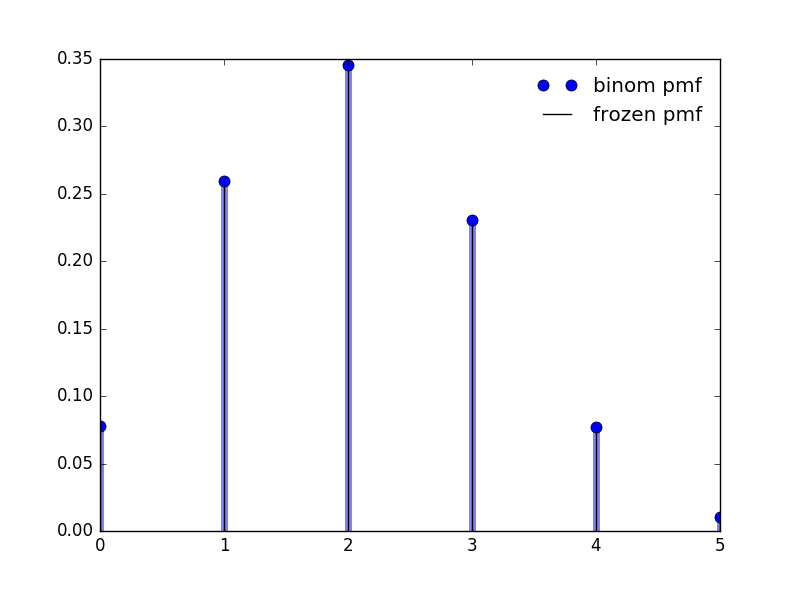
\includegraphics[width=0.6\textwidth]{../../img/math_probability/20160605binomDistribution.png}
\caption{\label{fig:org66d6bb2}
二项分布(5,0.4)的概率质量函数}
\end{figure}
\section{使用python做试验}
\label{sec:org9d8ed21}
\subsection{使用numpy}
\label{sec:orgd65fb9d}


python的第三方库 numpy 提供了丰富的随机变量相关的函数。

这里我们使用:
\lstset{language=Python,label= ,caption= ,captionpos=b,numbers=none}
\begin{lstlisting}
import numpy as np
\end{lstlisting}
导入numpy,在numpy下有 \texttt{numpy.random.binomial} 函数,这个函数:
\begin{verbatim}
Draw samples from a binomial distribution.
\end{verbatim}

生成10000个服从\((10,0.2)\)随机变量的样本。
\lstset{language=Python,label= ,caption= ,captionpos=b,numbers=none}
\begin{lstlisting}
s = numpy.random.binomial(10,0.5,10000)
\end{lstlisting}
我们知道服从二项分布\((10,0.5)\)的随机变量的期望是5,方差是2.5。

使用:
\lstset{language=Python,label= ,caption= ,captionpos=b,numbers=none}
\begin{lstlisting}
numpy.mean(s)
\end{lstlisting}
得到的输出是
\begin{verbatim}

In [243]: np.mean(s)
Out[246]:
4.9936999999999996

\end{verbatim}

这里为什么不是5?是因为取的样本太少的缘故。我们试着取一百万个样本:
\begin{verbatim}

In [247]: s  = np.random.binomial(10,.5,1000000)

In [251]: np.mean(s)
Out[258]:
5.0037690000000001

\end{verbatim}
可以看到均值还不严格的等于5,但是相对于一万个点得到的均值而言,一百万个样本点得到的均值更接近5.

使用 \texttt{numpy.var()} 可以查看样本点的方差。
\begin{verbatim}

In [261]: np.var(s)
Out[268]:
2.5008423010268426


\end{verbatim}

想象这样一个场景(这个例子来自于numpy.random.binomial的帮助文档)。一个石油勘探队挖10个井,每一个井出油的概率是0.1,那么挖了十个井后没有一个出油的概率是多大。我们可以从概率论的角度计算这个值:
\begin{equation}
\label{eq:13}
\binom{10}{0}(0.1)^{0}(0.9)^{10} = 0.348678
\end{equation}
当然我们也可以模拟100000次这样的试验,然后统计没有一个出油的频率,即在100000次试验中,这个随机变量取值为零的概率。
\lstset{language=Python,label= ,caption= ,captionpos=b,numbers=none}
\begin{lstlisting}
import numpy as np
s = np.random.binomial(10,0.1,100000)
sum(s == 0)/100000
\end{lstlisting}
我们得到的值是0.3491。

类似的,我们可以计算这个勘探队挖的这些井里有1个出油的概率。
\begin{equation}
\label{eq:14}
\binom{10}{1}(0.1)(0.9)^{9} = 0.38742
\end{equation}
我们实用100000次统计试验得出:
\lstset{language=Python,label= ,caption= ,captionpos=b,numbers=none}
\begin{lstlisting}
sum(s == 1)/100000
\end{lstlisting}
输出为0.38545.
依次类推我们可以计算:
\begin{eqnarray}
\label{eq:16}
p(n=2)&=&\binom{10}{2}(0.1)^{2}(0.9)^{8} = 0.1937  \\
p(n=3)&=&\binom{10}{3}(0.1)^{3}(0.9)^{7} = 0.05739 \\
p(n=4)&=&\binom{10}{4}(0.1)^{4}(0.9)^{6} = 0.01116  \\
p(n=5)&=&\binom{10}{5}(0.1)^{5}(0.9)^{5} = 0.001488 \\
p(n=6)&=&\binom{10}{6}(0.1)^{6}(0.9)^{4} = 0.00013778  \\
p(n=7)&=&\binom{10}{7}(0.1)^{7}(0.9)^{3} = 8.74\times 10^{-6}   \\
\end{eqnarray}
实用刚才的十万个样本点,我们可以得到:
\begin{verbatim}
sum(s == 2) / 100000 = 0.19411
sum(s == 3) / 100000 = 0.05804
sum(s == 4) / 100000 = 0.0116
sum(s == 5) / 100000 = 0.00167
sum(s == 6) / 100000 = 0.000149
sum(s == 7) / 100000 = 2e-5
\end{verbatim}
我们可以看到当\(n=7\)的时候我们的计算结果是\(8.74\times 10^{-6}\),但是统计得到的结果是\(2e-5\)。之所以出现如此大的差距是因为。样本点太小导致统计结果不准。对于较小的概率值\(p\)如果需要得到准确的估计,所需要的样本点大概是\(\frac{100}{p}\). 因此对于\(8.74\times 10^{-6}\)的概率值,我们需要大约\(8.74\times 10^{8}\)个样本点才可以比较准确的估计。

因为\(8.74\times 10^{8}\)实在是太大了,我的计算机受不了。我只好用10\^{}7个点来粗略的看看。
\begin{verbatim}

In [535]: s = np.random.binomial(10,0.1,10000000)

In [539]: sum(s == 7)/10000000
Out[555]:
9.0999999999999993e-06

\end{verbatim}
最后的估计值是\(9\times 10^{-6}\)。

我们希望画出服从\((n,p)\)的二项分布的图像,也就是式 (\ref{eq:16})。这个时候我们需要使用 scipy

\subsection{使用scipy}
\label{sec:org6e8d678}

Python的第三方安装包scipy提供了很多科学计算程序。比如,在式 (\ref{eq:16})中,我使用 \texttt{scipy.special.binom(N,n)} 来计算\(\binom{N}{n}\).

在scipy提供的众多科学计算程序中,也提供了很多统计学程序包。这些程序包放在 \texttt{scipy.stats} 下。注意导入stats需要使用 \texttt{from scipy import stats as S} .

然后,使 \texttt{S} 就和使用 \texttt{scipy.binom} 携带的一些列函数。

比如画出二项分布\((100,0.1)\)的概率质量函数是:
\lstset{language=Python,label= ,caption= ,captionpos=b,firstnumber=1,numbers=left}
\begin{lstlisting}
from scipy.stats import binom
import numpy as np
import matplotlib.pyplot as plt
from scipy import stats as S
N,p = 100,0.1
x = np.arange(0,N+1,1)
y = S.binom.pmf(x,N,p)
ax = plt.plot(x,y,'-bo');
plt.show()
\end{lstlisting}

\begin{figure}[htbp]
\centering
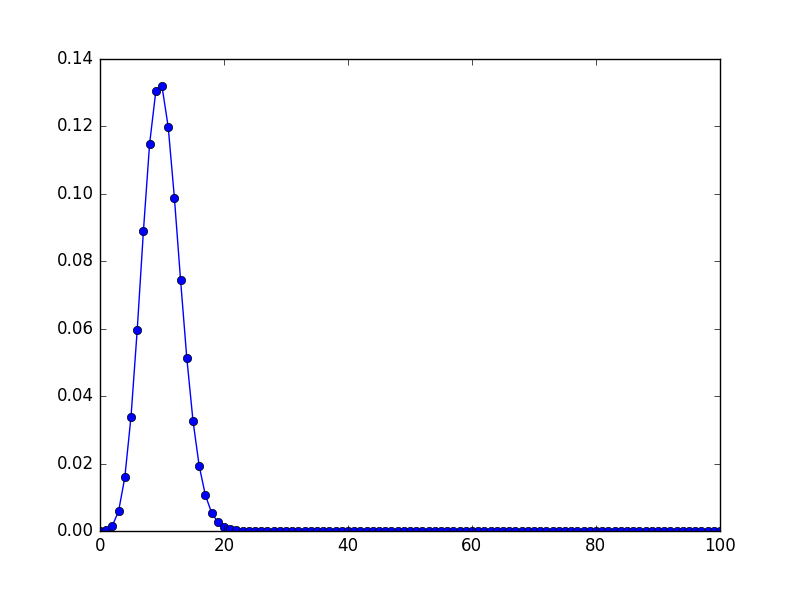
\includegraphics[width=0.6\textwidth]{../../img/math_probability/20170701binaryn100p0dot1.png}
\caption{\label{fig:orgfc1faea}
二项分布\((100,0.1)\)的概率质量函数}
\end{figure}

二项分布\((100,0.5)\)的概率质量函数,代码如下:
\lstset{language=Python,label= ,caption= ,captionpos=b,firstnumber=1,numbers=left}
\begin{lstlisting}
from scipy.stats import binom
import numpy as np
import matplotlib.pyplot as plt
from scipy import stats as S
N,p = 100,0.5
x = np.arange(0,N+1,1)
y = S.binom.pmf(x,N,p)
ax = plt.plot(x,y,'-bo');
plt.show()
\end{lstlisting}
图形如下
\begin{figure}[htbp]
\centering
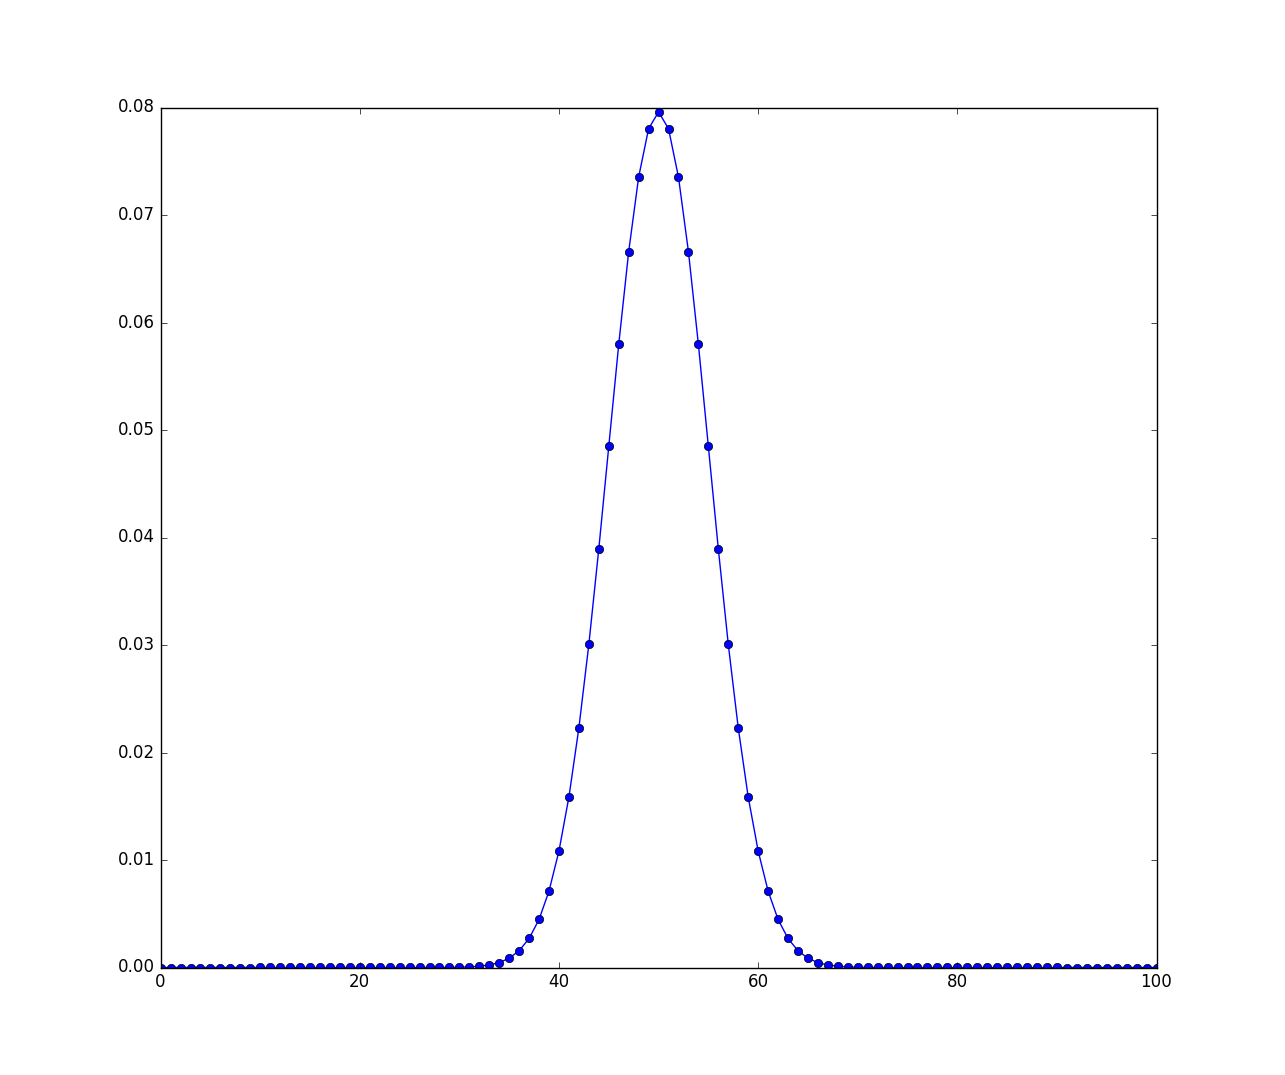
\includegraphics[width=0.6\textwidth]{../../img/math_probability/20170701binaryn100p0dot5.png}
\caption{\label{fig:org86630bf}
二项分布\((100,0.5)\)的概率质量函数}
\end{figure}
\end{document}
